\section{Introduction}
The evaluation of a predicted foreground map against a
ground-truth (GT) annotation map is crucial in evaluating
and comparing various computer vision algorithm for applications such as object detection\cite{borji2015salient,bylinskii2015saliency,kanan2010robust,qi2015saliencyrank} , saliency
prediction \cite{borji2014salient,hou2017deeply,jiang2013salient}, image segmentation and image collection browsing . As a
specific example, here we focus on salient object detection
models, although the proposed measure is general and can be used for other purposes. It is necessary to point out that the salient object is not necessary to be foreground object \cite{feng2016local}.

\section{Experimental Setup}

The experiments and related analysis are done in this chapter.It gives an assumption of the computation cost of finding visual saliency as well as a benchmark for comparing it to other existing method to find it's advantage and disadvantage. 
The experiments and analysis processes are done on a computer with Core-I3 processor having 2 cores with each core having 1.7GHz Speed. Also the system had 4GB of RAM, and 2 GB of intel hd video memory.
For software, Visual Studio 2015 Professional Edition is used and program is done with C++ language with OpenCV. OpenCV(Open Source Computer Vision) is a library of programming functions mainly aimed at real-time computer vision. It is developed by Intel’s research center at first and later maintained by Willow Garage and now is maintained by Itseez.
The reason for using OpenCV because it gives easy functionality to do different processes without going into implementations. Moreover it gives the benefit to use GPU by which processes can be made faster than using CPU only for computation works.

\subsection{Measuring Terms}

Saliency detection models often generate non-binary
maps. Traditional evaluation measures usually convert
these non-binary maps into multiple binary maps
\subsubsection{Evaluation of binary maps}

To evaluate a binary map,
four values are computed from the prediction confusion matrix: True Positives (TP), True Negatives (TN), False Positives (FP) and False Negatives (FN). These values are then
used to compute three ratios: True Positive Rate (TPR) or
Recall, False Positive Rate (FPR), and Precision.
To find these measures, 4 parameters are required to be known. They are described below:

\begin{enumerate}

\item True Positive: If predicted class is positive and the actual class is also positive then it is called True Positive.
\item True Negative: If predicted class is negative and the actual class is also negative then it is called True Negative.
\item False Positive: If predicted class is positive but the actual class is negative then it is called False Positive.
\item False Negative: If predicted class is negative but the actual class is positive then it is called False Negative.
\end{enumerate}
For example, if there 5 objects, 3 of them are actually Positive, 2 of them are actually negative, but 4 of them are predicted as Positive and 1 of them as negative them no of True Positive is 3, no of True Negative is 1, no of False Positive is 1 and no of False Negative 0.
Accuracy Accuracy is a measure that tells how much accurate the result is. It is expressed as such

\begin{align*}
 Accuracy&= \frac{TruePositive + TrueNegative}{TruePositive + TrueNegative + FalsePositive + FalseNegative}\\
 \end{align*}
\noindent
So accuracy is actually the ratio of the no of objects that are correctly classified divided by the total no of objects. For example, 50 percent accu- racy means 50 out of 100 data objects are correctly classified.
Precision Precision gives a measure that tells how much data objects are correctly and positively classified out of the all positively predicted data objects.

\begin{align*}
Precision &= \frac{TruePositive}{TruePositive + FalsePositive}\\
 \end{align*}
 So if precision is 25 percent,that means 25 data objects are correctly and positively classified out of 100 data objects that are predicted positively.
Recall Recall gives a measure that tells how much data objects are cor- rectly and positively classified out of the all actually positive data objects. It is expressed as such
\begin{align*}
Recall&=\frac{TruePositive}{TruePositive + FalseNegative}\\
 \end{align*} 
So if recall is 75 percent, that means 75 data objects are classified as Posi- tive out of 100 actually positive data objects. This measures give a positive feedback about the outcome, which means the more the values of these measures, the better the outcome is. But these measures might affect to each other. For example, increasing the amount of recall may cause decrease of precision because to increase recall, some portion of the non-foreground might come to the output as foreground, which can decrease the precision.

\subsubsection{Evaluation of non-binary maps}
PR- curve is
universally-agreed evaluation measures. Algorithms that
produce non-binary maps apply three steps to evaluate the agreement between model predictions (non-binary maps)
and human annotations (GT). First, multiple thresholds are
applied to the non-binary map to get multiple binary maps.
Second, these binary maps are compared to the binary mask
of the GT to get a set of TPR(True Positive Rate) & FPR(False Positive Rate) values. These values
are plotted in a 2D plot to get the PR curve.

\subsection{Dataset}
The  MSRA Salient Object Database \cite{cheng2015global}\cite{SalObjSurvey}\cite{SalObjBenchmark}\cite{13iccv/Cheng_Saliency}, which originally provides salient object annotation in terms of bounding boxes provided by 3-9 users, is widely used in salient object detection and segmentation community. Although an invaluable recourse to evaluate saliency detection algorithms, the database with the marked bounding boxes, however, is often too coarse for fine grained evaluation as observed by Wang and Li  \cite{wang2008two}and Achanta et al.\cite{achanta2010saliency}. In order to do more extensive and accurate evaluation, we randomly selected 10,000 images with consistent bounding box labeling in MSRA database. We call this dataset MSRA10K because it contains 10,000 images with pixel-level saliency labeling for 10K images from MSRA dataset.

\begin{figure}%
    \centering
    \subfloat[]{{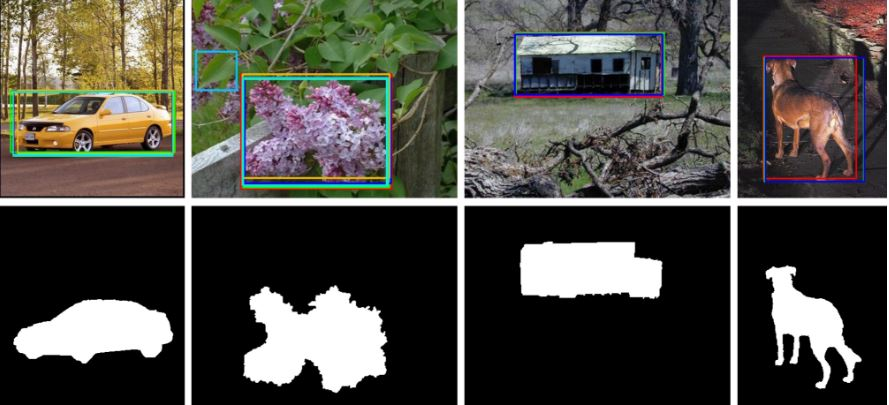
\includegraphics[width=0.6\textwidth,height=0.3\textwidth]{pictures/experiment/data1.jpg} }}%
    \caption{MSRA10k Dataset with Ground Truth and Original Image}%
    \label{fig:conversion23}%
\end{figure}


\subsection{Precision-Recall Curve}
For a saliency map S, we can
convert it to a binary mask M and compute P recision
and Recall by comparing M with ground-truth G.
The binarization
of S is the key step in the evaluation. Usually, there are
three popular ways to perform the binarization. In the first
solution, Achanta et al.\cite{achanta2010saliency} proposed the image-dependent
adaptive threshold for binarizing S, which is computed as
twice as the mean saliency of S.The second way to bipartite S is to use a fixed threshold
which changes from 0 to 255. On each threshold, a pair of precision/recall scores are computed, and are finally
combined to form a precision-recall (PR) curve to describe
the model performance at different situations.
The third way of binarization is to use the SaliencyCut
algorithm \cite{ren2014salient}. In this solution, a loose threshold, which
typically results in good recall but relatively poor precision,
is used to generate the initial binary mask. Then the method
iteratively uses the GrabCut segmentation method\cite{rother2004grabcut} to
gradually refines the binary mask. The final binary mask is
used to re-compute the precision-recall value.
We use the second way or Fixed-thresholding to measure the precision and recall.

\begin{figure}[here]%
    \centering
    \subfloat[]{{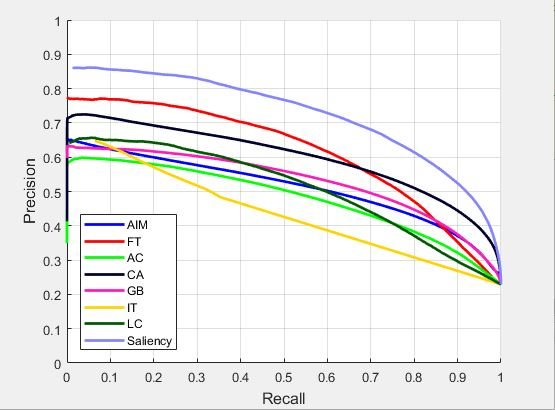
\includegraphics[width=0.7\textwidth,height=0.3\textwidth]{pictures/experiment/data.jpg} }}%
    \caption{Comparison with other method}%
    \label{fig:conversion23}%
\end{figure}
\noindent
From the figure it can be shown that saliency is way higher than other method IT\cite{itti1998model},GB\cite{harel2007graph},LC\cite{zhai2006visual},FT\cite{achanta2009frequency},AIM\cite{bruce2009saliency},CA\cite{goferman2012context}

\subsection{Mean Absolute Error}
The overlap-based
evaluation measures introduced like precision recall curve do not consider the
true negative saliency assignments, i.e., the pixels correctly
marked as non-salient. This favors methods that successfully assign saliency to salient pixels but fail to detect
non-salient regions over methods that successfully detect
non-salient pixels but make mistakes in determining the
salient ones. For a more comprehensive comparison we therefore
also evaluate the mean absolute error (MAE) between the
continuous saliency map S and the binary ground truth G,
both normalized in the range [0, 1]. The MAE score is
defined as:
\noindent
 
\begin{equation}\label{1}
MAE &= \frac{1}{W\times H} \sum_{x=1}^{W} \sum_{y=1}^{H}|S(x,y)-G(x,y)|
\end{equation}

\noindent
Here W is the width of the image and H is the height of the image. Following equation \ref{3} we get the MAE score as follows:
\begin{figure}[here]%
    \centering
    \subfloat[]{{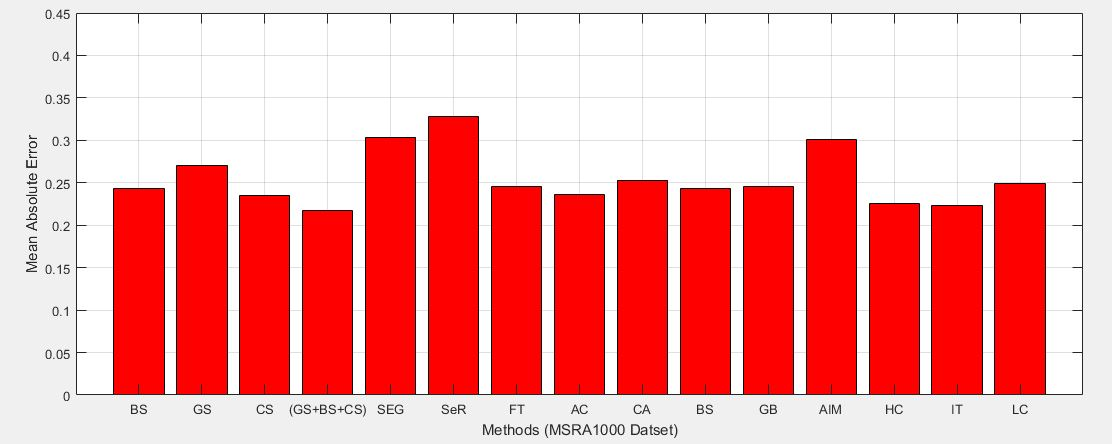
\includegraphics[width=1\textwidth,height=0.4\textwidth]{pictures/experiment/MSRAMAE.jpg} }}%
    \caption{Mean absolute error for MSRA1000 dataset}%
    \label{fig:conversion23}%
\end{figure}
\noindent


We can see that our saliency map combined of color saliency,boundary based saliency and global saliency has low MAE than other existing methods.